%==============================================================
% PF-3311 — Agentes Virtuales Inteligentes · Entregable 3
% Artículo académico (plantilla IEEE conference). Español.
% Compilar:  latexmk -pdf main.tex   (o subir a Overleaf)
%==============================================================
\documentclass[conference]{IEEEtran}
\IEEEoverridecommandlockouts

\usepackage[utf8]{inputenc}
\usepackage[T1]{fontenc}
\usepackage[spanish,es-noquoting]{babel}
\usepackage{graphicx}
\usepackage{booktabs}
\usepackage{amsmath}
\usepackage{url}
\usepackage{xcolor}
\usepackage{tikz}
\usetikzlibrary{positioning,arrows.meta,shapes.geometric,fit,backgrounds,calc}
\usepackage[hidelinks]{hyperref}

% Marcador visible para los datos empíricos que el estudio aún debe completar.
\newcommand{\todo}[1]{\textcolor{red}{\textbf{[PENDIENTE: #1]}}}

\begin{document}

\title{Sonic: un tutor socr\'atico multimodal corporizado para el desarrollo de l\'ogica de programaci\'on en entornos STEM}

\author{\IEEEauthorblockN{Gabriel Isa\'ias Fallas L\'opez}
\IEEEauthorblockA{Escuela de Ciencias de la Computaci\'on e Inform\'atica\\
Universidad de Costa Rica\\
San Jos\'e, Costa Rica\\
gabrielfallas0803@gmail.com}}

\maketitle

\begin{abstract}
La integraci\'on masiva de modelos de lenguaje (LLMs) en la educaci\'on en computaci\'on
ha generado una paradoja pedag\'ogica: el acceso inmediato a soluciones de c\'odigo erosiona
el desarrollo del razonamiento l\'ogico y la descomposici\'on de problemas. Este art\'iculo
presenta \emph{Sonic}, un tutor socr\'atico que gu\'ia al estudiante mediante preguntas
reflexivas y andamiaje graduado (Zona de Desarrollo Pr\'oximo) sin entregar c\'odigo directo.
El sistema se implementa sobre un LLM local (Ollama + Gemma~3 12B) y se eval\'ua mediante un
\emph{estudio piloto} de dos condiciones: una condici\'on corporizada (A) con avatar 2D reactivo
(Kaplay.js), s\'intesis de voz neuronal (Piper~TTS), reconocimiento de voz local (Whisper~STT) y
gamificaci\'on por anillos; y una condici\'on de control (B) de chat de texto plano con
\emph{id\'entico} tutor socr\'atico. Mediante tareas de depuraci\'on en Python verificadas por
pruebas ocultas, se miden la eficacia aut\'onoma, la carga cognitiva (NASA-TLX), la percepci\'on
del agente (Godspeed), la usabilidad (SUS), el afecto post-sesi\'on (PANAS-SF) y un conjunto de
m\'etricas conductuales autom\'aticas (latencia, turnos, tiempo de reflexi\'on, uso de voz).
En un estudio piloto de $N=10$ participantes (6 entre-sujetos y 4 intra-sujeto, que aportan 14
observaciones, 7 por condici\'on), la condici\'on corporizada obtuvo puntuaciones de percepci\'on
del agente marcadamente superiores (Godspeed global $d=1{,}42$; subescala de agrado $d=1{,}66$,
\mbox{$p=0{,}011$}) y una carga cognitiva autopercibida menor (NASA-TLX $d=-0{,}83$), con
usabilidad (SUS) ligeramente mejor y eficacia de resoluci\'on equivalente; el
\emph{time-to-first-token} se mantuvo bajo 1.5~s en el 92\,\% de las respuestas. El an\'alisis
cualitativo refuerza el patr\'on: varios participantes ---incluidos quienes experimentaron ambas
condiciones--- prefirieron expl\'icitamente el avatar sobre el texto. Dado el tama\~no muestral,
los resultados son preliminares y se reportan como tama\~nos de efecto. Los hallazgos contribuyen a
comprender el rol del \emph{embodiment} en tutores socr\'aticos para programaci\'on y su efecto
sobre la autonom\'ia del aprendiz.
\end{abstract}

\begin{IEEEkeywords}
tutor\'ia socr\'atica, agentes virtuales corporizados, modelos de lenguaje, andamiaje
cognitivo, educaci\'on en programaci\'on, gamificaci\'on.
\end{IEEEkeywords}

%--------------------------------------------------------------
\section{Introducci\'on}
La educaci\'on en ciencias, tecnolog\'ia, ingenier\'ia y matem\'aticas (STEM) atraviesa una
transformaci\'on impulsada por la IA generativa. En computaci\'on, la disponibilidad inmediata
de soluciones de c\'odigo produce una \emph{descarga cognitiva}: el estudiante delega la
resoluci\'on de errores l\'ogicos a un sistema que devuelve el c\'odigo corregido, eliminando el
proceso de prueba y error esencial para formar modelos mentales robustos~\cite{phung2023generative,raihan2025llms}.
El m\'etodo socr\'atico ---no proporcionar la respuesta, sino guiar mediante preguntas que
revelan contradicciones y lagunas--- es un ant\'idoto reconocido, pero su escalabilidad es nula
en cursos con cientos de estudiantes.

Este trabajo investiga si un tutor socr\'atico basado en LLM, dotado de \emph{corporizaci\'on}
multimodal (avatar reactivo, voz neuronal, reconocimiento de voz y gamificaci\'on), mejora la
percepci\'on del agente y la eficacia pedag\'ogica aut\'onoma frente al mismo tutor en modo de
texto plano. La contribuci\'on es triple: (i) un sistema reproducible, completamente local y
sin dependencias de nube; (ii) un dise\~no experimental que a\'isla el \emph{embodiment}
manteniendo constante el texto del tutor; y (iii) un conjunto de m\'etricas conductuales
autom\'aticas que reduce la dependencia del auto-reporte.

El resto del art\'iculo se organiza as\'i: la Secci\'on~\ref{sec:related} revisa los trabajos
relacionados; la Secci\'on~\ref{sec:agent} describe el desarrollo del agente; la
Secci\'on~\ref{sec:method} detalla la metodolog\'ia; las Secciones~\ref{sec:results}
y~\ref{sec:discussion} presentan y discuten los resultados; y la Secci\'on~\ref{sec:conclusion}
concluye.

%--------------------------------------------------------------
\section{Trabajos Relacionados}
\label{sec:related}

\subsection{IA generativa y descarga cognitiva en programaci\'on}
La irrupci\'on de asistentes de c\'odigo basados en LLM transform\'o la pr\'actica de aprender a
programar. Phung et al.~\cite{phung2023generative} documentan tanto el potencial de estos modelos
para generar retroalimentaci\'on como su capacidad de resolver directamente los ejercicios, y
Raihan et al.~\cite{raihan2025llms} sintetizan su uso en educaci\'on en computaci\'on. El riesgo
pedag\'ogico es la \emph{descarga cognitiva}: si el sistema devuelve la soluci\'on, el estudiante
omite el ciclo de prueba, error y depuraci\'on del que dependen los modelos mentales robustos. De
ah\'i el inter\'es por reorientar estos modelos de ``solucionadores'' a ``tutores'' que retienen la
respuesta.

\subsection{Tutor\'ia socr\'atica con modelos de lenguaje}
El m\'etodo socr\'atico ---guiar mediante preguntas en lugar de dar la respuesta--- se ha vuelto un
patr\'on recurrente para esa reorientaci\'on. \emph{SocraticLM}~\cite{liu2024socraticlm} y
\emph{SocraticAI}~\cite{sunil2025socraticai} estructuran la interacci\'on en niveles de andamiaje
progresivo; \emph{MathDial}~\cite{macina2023mathdial} aporta un corpus de di\'alogos tutoriales con
propiedades pedag\'ogicas ricas que sirve de referencia para entrenar y evaluar; y Jurenka et
al.~\cite{jurenka2024problem} alinean el modelo con objetivos pedag\'ogicos para sostener la
indagaci\'on sin revelar la soluci\'on. En el plano de la evaluaci\'on, Tack y
Piech~\cite{tack2022clean} proponen criterios para juzgar la calidad tutorial de un agente, un
problema no trivial dado que ``parecer'' un buen tutor no implica producir aprendizaje. Estudios
m\'as recientes reportan ganancias de aprendizaje, compromiso metacognitivo y mejor percepci\'on
del andamiaje en cursos STEM introductorios~\cite{ali2026tool,xi2026investigating,kao2025socratic},
y Essel et al.~\cite{essel2024aimediated} vinculan espec\'ificamente el cuestionamiento mediado por
IA con el compromiso del estudiante ---trabajo del que adaptamos nuestra escala de apoyo
pedag\'ogico. Una limitaci\'on transversal es que la \emph{planificaci\'on adaptativa} del di\'alogo
(decidir cu\'ando y cu\'anto andamiar) sigue siendo incipiente~\cite{dong2026learning}; nuestro
sistema adopta una pol\'itica simple y expl\'icita de tres niveles ligada al estancamiento del
estudiante.

\subsection{Agentes conversacionales corporizados en educaci\'on}
M\'as all\'a del texto, una l\'inea de trabajo dota al tutor de un cuerpo ---avatar, voz, gestos.
La revisi\'on de alcance de Sonlu et al.~\cite{sonlu2024scoping} sintetiza una d\'ecada de agentes
conversacionales corporizados y concluye que la \emph{presencia social} suele mejorar la
experiencia, pero con resultados heterog\'eneos seg\'un la tarea, la poblaci\'on y el grado de
realismo. En programaci\'on y entornos inmersivos, propuestas multimodales y de realidad
virtual~\cite{elhajji2025architecture,yang2025embodied} sugieren que la corporizaci\'on puede
favorecer el aprendizaje y la motivaci\'on, aunque advierten dos riesgos: una carga perceptiva
adicional y el rechazo cuando el realismo es casi-humano pero imperfecto (\emph{Valle Inquietante})
~\cite{mori1970uncanny}. Nuestro uso de un personaje estilizado y reconocible (un sprite 2D) en
lugar de un humano fotorrealista es, en parte, una respuesta a este \'ultimo riesgo.

\subsection{Carga cognitiva, novedad y medici\'on}
La evidencia agregada invita a la cautela. El meta-an\'alisis de Xu et al.~\cite{xu2026educationalagents}
estima un efecto \emph{positivo pero peque\~no} de los agentes pedag\'ogicos sobre el aprendizaje, y
el de Li et al.~\cite{li2025cognitiveload} muestra que solo reducen levemente la carga cognitiva e
incluso la \emph{aumentan} en materiales complejos o sesiones largas ---un riesgo directamente
pertinente para una tarea densa como la depuraci\'on. A ello se suma que las medidas de auto-reporte
y las conductuales correlacionan d\'ebilmente~\cite{dang2020selfreport}, por lo que apoyarse solo en
cuestionarios puede inducir conclusiones fr\'agiles, especialmente con muestras peque\~nas. Estos
hallazgos motivan nuestras decisiones metodol\'ogicas: medir la carga (NASA-TLX) y el afecto
(PANAS-SF) con instrumentos validados, complementarlos con telemetr\'ia conductual objetiva, y
tratar el atractivo inicial del personaje como un posible \emph{efecto de novedad} a controlar.

\subsection{Brecha y posicionamiento}
En conjunto, la literatura aborda por separado (a) la calidad socr\'atica del di\'alogo y (b) el
efecto de la corporizaci\'on, y con frecuencia compara condiciones cuyo \emph{contenido} de tutor
difiere, lo que confunde el efecto del \emph{embodiment} con el de una persona o un guion distinto.
Adem\'as, la eficacia suele medirse por auto-reporte. Este trabajo se posiciona en esa brecha en
tres puntos: (i)~compara dos condiciones con \emph{texto de tutor id\'entico}, aislando el
\emph{embodiment} (avatar + voz + gamificaci\'on); (ii)~mide la eficacia aut\'onoma con
verificaci\'on \emph{objetiva} (pruebas ocultas) en lugar de auto-reporte; y (iii)~combina
auto-reporte, telemetr\'ia conductual y an\'alisis cualitativo para sortear la d\'ebil correlaci\'on
entre tipos de medida.

%--------------------------------------------------------------
\section{Desarrollo del Agente}
\label{sec:agent}

\subsection{Arquitectura del sistema}
El sistema es una aplicaci\'on web \textbf{Next.js 15} (App Router, React~19, TypeScript) cuyos
servicios de IA corren \emph{en local}, sin claves de API ni dependencias de nube
(Fig.~\ref{fig:arch}). Se organiza en tres capas: (i)~un \textbf{cliente} en el navegador con el
panel de c\'odigo, el chat, el avatar y la voz; (ii)~un \textbf{servidor} Next.js que expone rutas
de API y orquesta la inferencia; y (iii)~tres \textbf{servicios locales} ---el modelo de lenguaje,
la s\'intesis y el reconocimiento de voz--- m\'as una base de datos embebida para la telemetr\'ia.

\begin{figure}[t]
  \centering
  \footnotesize
  \begin{tikzpicture}[
    node distance=3.2mm,
    box/.style={draw, rounded corners=2pt, align=center, inner sep=2.6pt, font=\scriptsize, minimum height=6.5mm},
    cli/.style={box, fill=blue!8},
    srv/.style={box, fill=orange!12},
    svc/.style={box, fill=green!10},
    lbl/.style={font=\scriptsize\bfseries},
    >={Stealth[length=1.6mm]}]
    % Client tier
    \node[cli] (code) {Panel de c\'odigo\\(Pyodide \emph{worker})};
    \node[cli, right=of code] (chat) {Chat socr\'atico};
    \node[cli, right=of chat] (avatar) {Avatar Kaplay\\+ anillos};
    \node[cli, right=of avatar] (voice) {Voz\\(TTS/STT)};
    \node[lbl, left=2mm of code] (climbl) {Cliente};
    \begin{scope}[on background layer]
      \node[draw, dashed, rounded corners, fit=(climbl)(code)(chat)(avatar)(voice), inner sep=2.2mm] (clitier) {};
    \end{scope}
    % Server tier
    \node[srv, below=10mm of chat] (chatapi) {\texttt{/api/chat}\\(SSE \emph{streaming})};
    \node[srv, left=of chatapi] (sessapi) {\texttt{/api/session}};
    \node[srv, right=of chatapi] (sttapi) {\texttt{/api/stt}};
    \node[lbl, left=2mm of sessapi] (srvlbl) {Servidor};
    \begin{scope}[on background layer]
      \node[draw, dashed, rounded corners, fit=(srvlbl)(sessapi)(chatapi)(sttapi), inner sep=2.2mm] (srvtier) {};
    \end{scope}
    % Service tier
    \node[svc, below=10mm of sessapi] (db) {SQLite\\\texttt{sonic.db}};
    \node[svc, right=of db] (ollama) {Ollama\\Gemma~3 12B};
    \node[svc, right=of ollama] (piper) {Piper TTS};
    \node[svc, right=of piper] (whisper) {Whisper STT};
    \node[lbl, left=2mm of db] {Servicios locales};
    % edges
    \draw[<->] (chat) -- (chatapi);
    \draw[<->] (code.south) -- ++(0,-3mm) -| (sessapi.north);
    \draw[<->] (voice.south) -- ++(0,-3mm) -| (sttapi.north);
    \draw[<->] (chatapi) -- (ollama);
    \draw[<->] (sessapi) -- (db);
    \draw[<->] (sttapi) -- (whisper);
    \draw[<->] (voice.east) to[out=-20,in=20] (piper.north east);
  \end{tikzpicture}
  \caption{Arquitectura en tres capas. El texto del tutor es id\'entico en ambas condiciones; el
  avatar, la voz y la gamificaci\'on (sombreado) solo se activan en la Condici\'on~A.}
  \label{fig:arch}
\end{figure}

Los componentes principales son:
\begin{itemize}
  \item \textbf{Motor de razonamiento.} Ollama sirve a Gemma~3 12B (cuantizaci\'on Q4\_K\_M,
        inferencia en GPU local). La ruta \texttt{/api/chat} construye el \emph{system prompt}
        socr\'atico, env\'ia el historial al modelo y retransmite la respuesta al cliente por
        \emph{streaming} de tokens (Server-Sent Events) para minimizar la latencia percibida
        (objetivo $<1.5$~s de \emph{time-to-first-token}).
  \item \textbf{Avatar 2D (Condici\'on A).} Un \emph{canvas} Kaplay.js renderiza un sprite reactivo
        con \textbf{ocho estados expresivos}; su control se detalla en la
        Secci\'on~\ref{sec:scaffold}.
  \item \textbf{Voz (Condici\'on A).} S\'intesis neuronal Piper~TTS (espa\~nol) con respaldo a la
        Web Speech API; reconocimiento de voz local Whisper~STT v\'ia \texttt{/api/stt}.
  \item \textbf{Gamificaci\'on (Condici\'on A).} Sistema de anillos (recompensa al acertar),
        mini-juego de transici\'on entre tareas y efectos de sonido/m\'usica por zona tem\'atica.
  \item \textbf{Ejecuci\'on de c\'odigo.} Un editor real ejecuta Python en el navegador (Pyodide en
        un \emph{Web Worker} con \emph{timeout}) y anexa un arn\'es de pruebas ocultas que
        determina objetivamente la resoluci\'on aut\'onoma.
  \item \textbf{Telemetr\'ia.} Persistencia en una base SQLite embebida; exportaci\'on a
        CSV/JSON/transcripciones y panel del facilitador (Secci\'on~\ref{sec:telemetry}).
\end{itemize}

\subsection{Andamiaje socr\'atico y control afectivo del avatar}
\label{sec:scaffold}
El comportamiento pedag\'ogico se especifica en un \emph{system prompt} compartido por ambas
condiciones, con tres reglas duras: no generar ni corregir c\'odigo, no se\~nalar la l\'inea
err\'onea, y terminar siempre con una pregunta reflexiva (respuestas de 3--4 oraciones, sin
emojis). El conocimiento del error real se entrega al modelo solo para razonar, nunca para
revelarlo.

\paragraph{Tres niveles de andamiaje (ZPD)} Operacionalizando la Zona de Desarrollo
Pr\'oximo~\cite{vygotsky1978mind}, la ayuda escala \emph{solo} si el estudiante acumula tres o m\'as
turnos sin avanzar:
\begin{itemize}
  \item \textbf{Nivel 1 (turnos 1--2): preguntas amplias} sobre el objetivo del c\'odigo
        (p.\,ej.\ ``¿qu\'e condici\'on debe volverse falsa para que el bucle se detenga?'').
  \item \textbf{Nivel 2 (turnos 3--4): orientaci\'on conceptual} hacia la estructura o el invariante
        (p.\,ej.\ ``¿qu\'e valor tiene esa variable en la primera iteraci\'on frente a la
        segunda?'').
  \item \textbf{Nivel 3 (turnos 5+): pista estructural, todav\'ia sin c\'odigo}, dirigiendo la
        atenci\'on a la l\'inea o a la complejidad (``si la lista tiene $N$ elementos, ¿cu\'antas
        comparaciones hace tu algoritmo?'').
\end{itemize}

\paragraph{Detecci\'on de estado afectivo} El sistema combina dos mecanismos. Primero, una
\emph{regla de des-escalada}: ante marcadores l\'exicos de frustraci\'on (``no entiendo'', ``no
s\'e'', ``me rindo'', ``ayuda'', ``no puedo'') el tutor valida el esfuerzo, retrocede un nivel de
andamiaje y pide reformular el problema en palabras simples. Segundo, una \emph{inferencia
afectiva} que el propio modelo realiza sobre el turno del estudiante para seleccionar el estado
expresivo del avatar. Estos estados se transmiten mediante una etiqueta
\texttt{[AVATAR\_STATE:\,estado]} que el modelo a\~nade al final de la respuesta (Condici\'on~A) y
que el cliente \emph{elimina} antes de mostrar el texto, de modo que la transcripci\'on visible es
id\'entica a la de la Condici\'on~B. Los ocho estados son: cuatro \emph{inferidos por el modelo}
seg\'un el contenido ---\textbf{curious} (pregunta reflexiva, por defecto), \textbf{happy}
(el estudiante se acerca a la soluci\'on), \textbf{empathetic} (frustraci\'on) y
\textbf{encouraging} (motivar a seguir)--- y cuatro \emph{dirigidos por eventos de interacci\'on}
en el cliente ---\textbf{thinking} (mientras se genera la respuesta), \textbf{speaking} (durante la
locuci\'on TTS), \textbf{listening} (durante la captura de voz/espera) e \textbf{idle} (reposo).
As\'i, el avatar reacciona tanto al \emph{qu\'e} dice el estudiante como al \emph{momento} de la
interacci\'on.

\subsection{Decisi\'on de dise\~no clave: aislar el \emph{embodiment}}
Ambas condiciones comparten el \emph{mismo} texto de tutor; la \'unica diferencia a nivel de
\emph{prompt} es el bloque de control del avatar a\~nadido en la Condici\'on~A (cuya \'unica salida,
la etiqueta de estado, se elimina antes de mostrarse). As\'i, la comparaci\'on A vs.\ B mide el
efecto de la corporizaci\'on (sprite + voz + gamificaci\'on) y no una persona o un texto distinto.
Las Figuras~\ref{fig:condA} y~\ref{fig:condB} muestran ambas interfaces.

\begin{figure}[t]
  \centering
  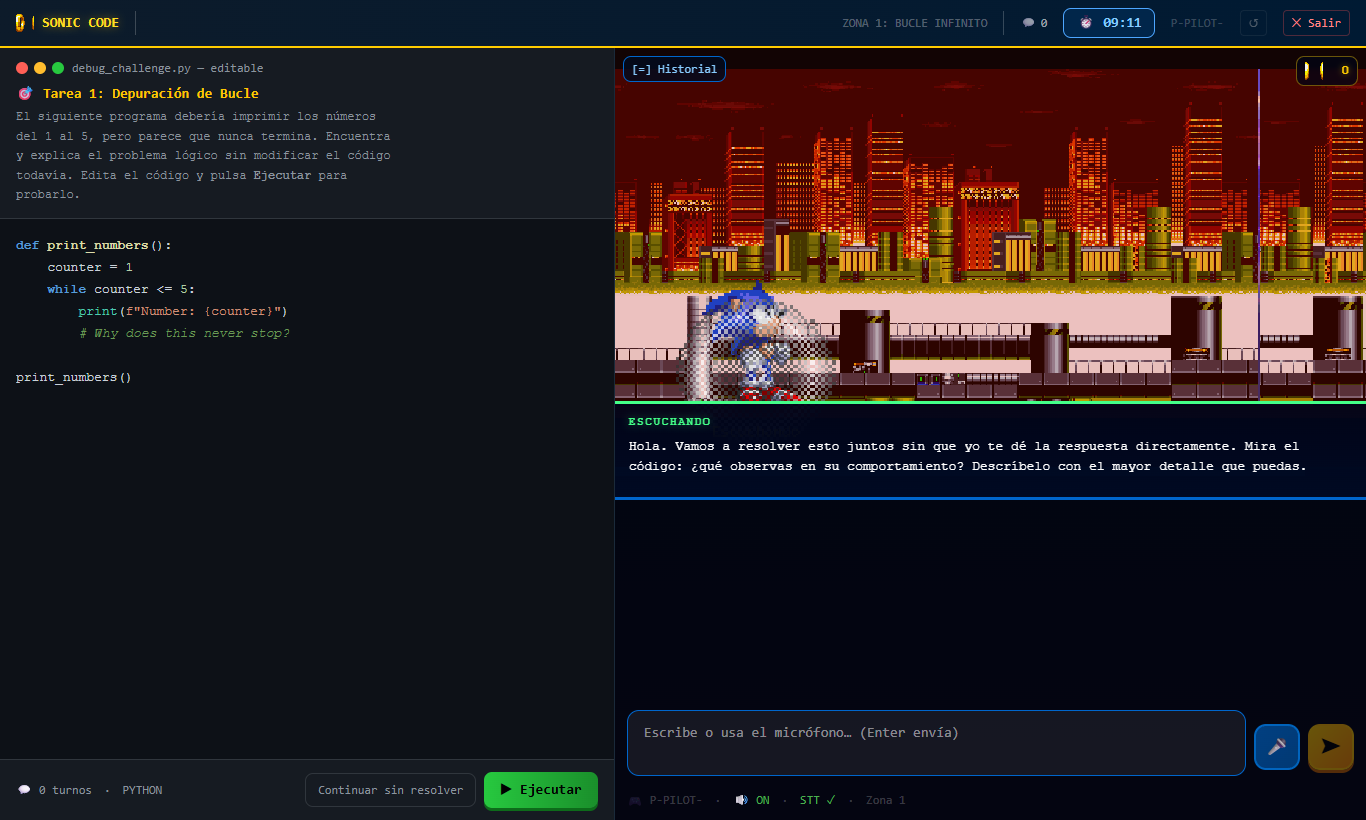
\includegraphics[width=\columnwidth]{figures/condA-initial.png}
  \caption{Condici\'on A (corporizada): avatar Sonic en \emph{canvas} Kaplay.js, HUD de anillos y
  panel de c\'odigo con ejecuci\'on en Pyodide.}
  \label{fig:condA}
\end{figure}

\begin{figure}[t]
  \centering
  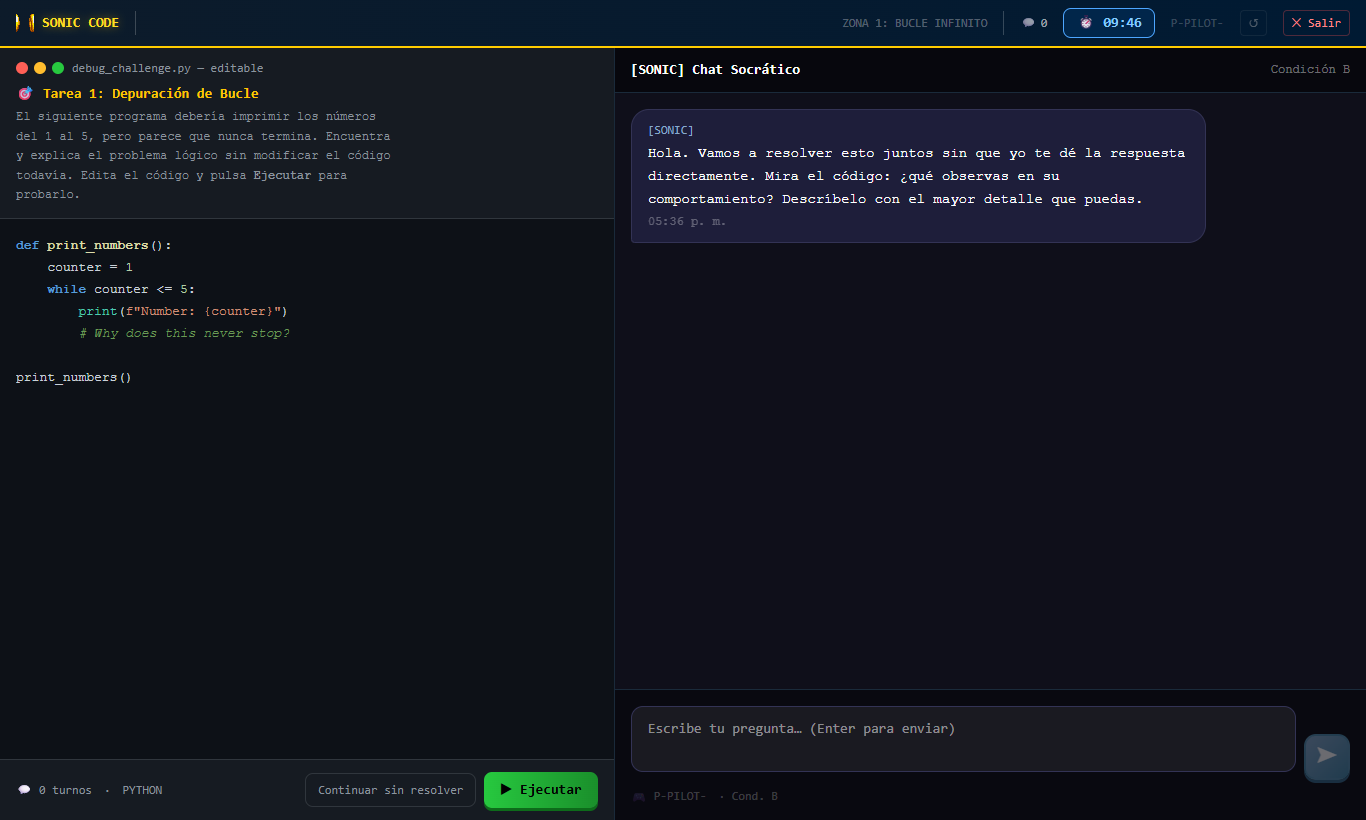
\includegraphics[width=\columnwidth]{figures/condB-initial.png}
  \caption{Condici\'on B (control): chat de texto plano con el mismo tutor socr\'atico, sin
  avatar, voz ni gamificaci\'on.}
  \label{fig:condB}
\end{figure}

\subsection{Telemetr\'ia y datos registrados}
\label{sec:telemetry}
Toda la sesi\'on se persiste en una base SQLite embebida (\texttt{sonic.db}) anclada a la ra\'iz del
proyecto. El esquema tiene cuatro tablas: \texttt{sessions} (una fila por participante con el
registro completo en JSON m\'as columnas indexadas \texttt{condition}/\texttt{isPilot}/tiempos),
\texttt{events} (bit\'acora append-only de hitos: inicio, resultado de tarea, cuestionario, cierre),
\texttt{assignment} (contador de contrabalanceo persistente, para que la numeraci\'on
P-001\dots\ y el balance A/B sobrevivan reinicios) y \texttt{meta}. Por cada sesi\'on se
almacenan, y se usan as\'i:
\begin{itemize}
  \item \textbf{Mensajes:} rol, contenido, marca de tiempo, \texttt{inputMode} (voz/teclado) y
        \texttt{latencyMs}/\texttt{ttftMs} por respuesta del tutor. Sirven para la latencia (RQ4),
        el \emph{think-time} entre turnos (reflexi\'on, RQ2), la verbosidad y el uso de voz (RQ1).
  \item \textbf{Resultados de tarea:} \texttt{resolvedAutonomously} y \texttt{testsPassed} (eficacia
        objetiva, RQ2), \texttt{turns}, \texttt{timeSpentSeconds}, \texttt{codeRunAttempts} y
        \texttt{codeEdited} (esfuerzo y proceso), \texttt{ringsCollected} (compromiso gamificado) y
        la \texttt{condition} de esa tarea (clave del dise\~no \emph{crossover}).
  \item \textbf{Cuestionarios:} respuestas crudas y puntajes derivados por instrumento, etiquetados
        por condici\'on, que alimentan RQ1 (Godspeed, apoyo pedag\'ogico, SUS) y RQ3 (NASA-TLX,
        PANAS-SF).
  \item \textbf{Metadatos del dise\~no:} \texttt{design}, \texttt{sequence} y los tiempos de
        inicio/cierre, que permiten combinar las observaciones entre-sujetos y \emph{crossover}.
\end{itemize}
Tres exportaciones derivan de esta base: un CSV con una fila por participante (m\'etricas y
puntajes), un JSON de fidelidad completa y las transcripciones en JSONL para codificaci\'on
cualitativa.

\subsection{Implementaci\'on}
El cliente y el servidor se construyeron como una \'unica aplicaci\'on Next.js con renderizado del
lado del cliente para las vistas interactivas. El \textbf{chat} mantiene el historial en React y
consume \texttt{/api/chat}, que abre una conexi\'on SSE: el servidor invoca a Ollama, lee el flujo
de tokens y los reenv\'ia conforme llegan, midiendo el \emph{time-to-first-token} en el primer
fragmento. El \textbf{panel de c\'odigo} integra un editor y un \emph{Web Worker} que inicializa
Pyodide una sola vez; al ejecutar, concatena el c\'odigo del estudiante con el arn\'es de pruebas
oculto y captura la l\'inea \texttt{\_\_TESTS\_\_} que reporta \emph{passed}/\emph{detail}, con un
\emph{timeout} que sirve adem\'as para detectar bucles infinitos (Fig.~\ref{fig:pyodide}). El
\textbf{avatar} se dibuja en un \emph{canvas} Kaplay.js independiente; la \textbf{voz} usa el
endpoint \texttt{/api/stt} (Whisper) para transcribir y Piper para sintetizar la respuesta. La
\textbf{asignaci\'on} de condici\'on/orden se resuelve en el servidor por bloques permutados y se
persiste, evitando que el participante elija condici\'on. Las \textbf{tareas} de depuraci\'on son:
(T1) un bucle \texttt{while} que no termina por un contador que no se actualiza; y (T2) un
algoritmo de fuerza bruta con bucles anidados que debe optimizarse a $O(n)$ con un conjunto; para el dise\~no \emph{crossover}
existe una segunda variante equivalente de cada una. Todo el sistema se empaqueta con Docker
Compose (la aplicaci\'on, Ollama y el servicio de voz) para una ejecuci\'on reproducible con un solo
comando.

\begin{figure}[t]
  \centering
  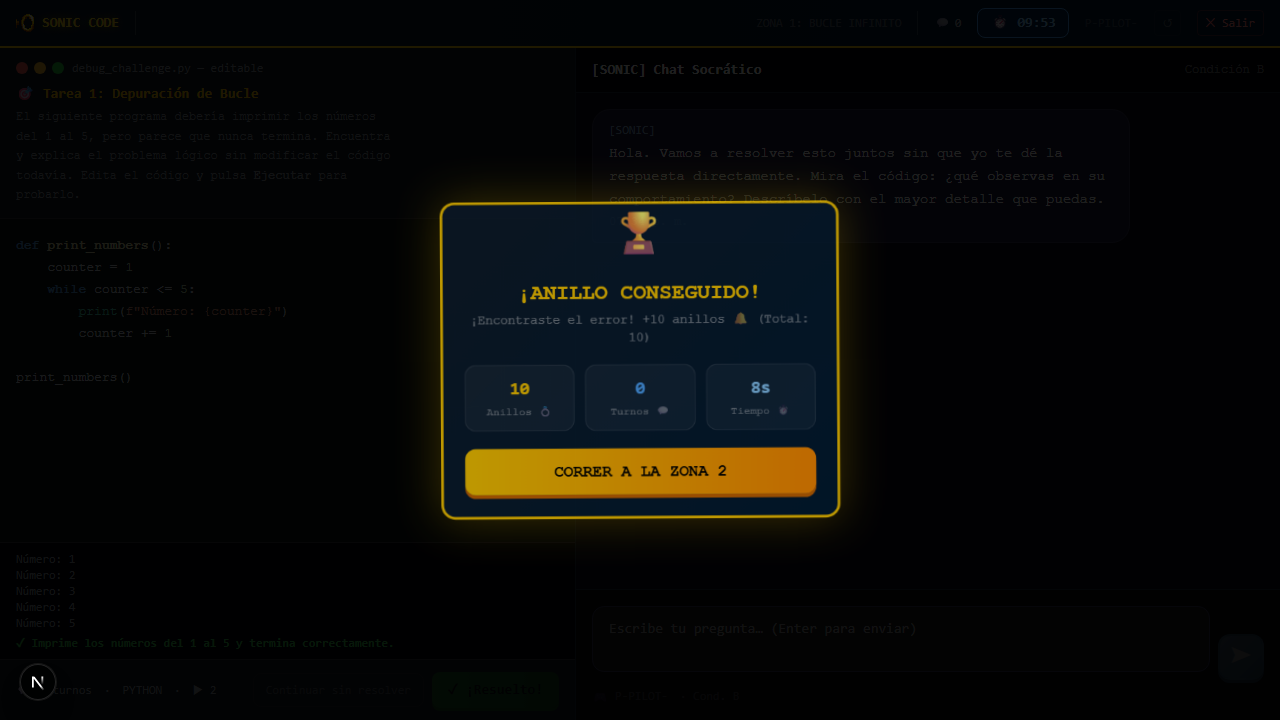
\includegraphics[width=\columnwidth]{figures/pyodide-fixed.png}
  \caption{Verificaci\'on objetiva de la resoluci\'on: el arn\'es de pruebas ocultas confirma que
  la correcci\'on del estudiante pasa.}
  \label{fig:pyodide}
\end{figure}

\begin{figure}[t]
  \centering
  
\includegraphics[width=\columnwidth]{figures/landing.png}
  \caption{Pantalla de inicio. El participante pulsa \emph{PRESS START} y el servidor asigna la
  condici\'on/orden; los botones de prueba quedan ocultos durante la recolecci\'on real.}
  \label{fig:landing}
\end{figure}

%--------------------------------------------------------------
\section{Metodolog\'ia}
\label{sec:method}

\subsection{Preguntas de investigaci\'on}
\begin{itemize}
  \item \textbf{RQ1.} ¿C\'omo afecta la corporizaci\'on a la percepci\'on de naturalidad,
        presencia social y apoyo pedag\'ogico percibido?
  \item \textbf{RQ2.} ¿En qu\'e medida la modalidad influye en la eficacia pedag\'ogica
        aut\'onoma (resoluci\'on sin c\'odigo directo, turnos, tiempo)?
  \item \textbf{RQ3.} ¿Qu\'e relaci\'on existe entre la modalidad y la carga cognitiva (NASA-TLX)
        y el afecto post-sesi\'on (PANAS-SF)?
  \item \textbf{RQ4.} ¿Se mantiene la latencia multimodal por debajo de 1.5~s de forma
        consistente?
\end{itemize}

\subsection{Dise\~no del estudio}
Este art\'iculo reporta un \emph{estudio piloto de viabilidad} ejecutado en dos fases con un
dise\~no mixto. La \textbf{Fase~1} (6 participantes) emple\'o un dise\~no \textbf{entre-sujetos}:
cada participante se asign\'o a \emph{una} condici\'on (A corporizada o B texto) y resolvi\'o en
ella las dos tareas de depuraci\'on. La \textbf{Fase~2} (4 participantes) emple\'o un dise\~no
\textbf{intra-sujeto (\emph{crossover})}, en el que cada participante resolvi\'o ambas tareas en
\emph{ambas} condiciones. En ambas fases la asignaci\'on (de condici\'on o de orden) la realiza el
servidor mediante \emph{aleatorizaci\'on por bloques permutados}, de modo que el participante nunca
elige su condici\'on y el balance A/B queda garantizado por bloque. Se adopta un esquema
\emph{post-only}: \textbf{no se administran formularios al inicio} ---el participante entra directo
a la experiencia--- lo que reduce la fricci\'on inicial y evita el \emph{priming} de medidas
previas. Como cada sesi\'on \emph{crossover} aporta una observaci\'on por condici\'on y cada sesi\'on
entre-sujetos aporta una, ambos dise\~nos se combinan en el contraste A vs.\ B por condici\'on
(14~observaciones; 7 por condici\'on).

\paragraph{Dise\~no \emph{crossover} con variantes de tarea}
En la Fase~2, cada participante realiza cuatro ejercicios en dos bloques (las dos tareas en una
condici\'on y luego en la opuesta), con el \emph{orden} de condiciones contrabalanceado (A$\to$B /
B$\to$A). Para evitar que el participante resuelva el problema id\'entico dos veces (efecto de
pr\'actica/memoria ---se\~nalado por un participante de la Fase~1), cada tarea tiene \textbf{dos
variantes equivalentes} en dificultad y constructo (dos errores de terminaci\'on de bucle
distintos; dos algoritmos de fuerza bruta con bucles anidados optimizables a $O(n)$ con un \emph{set}): el Bloque~1 usa la
variante~1 y el Bloque~2 la variante~2. Como la variante est\'a ligada a la posici\'on del bloque y
el orden de condiciones es contrabalanceado, la dificultad de variante queda balanceada entre A y
B. El dise\~no intra-sujeto controla las diferencias individuales y maximiza la potencia con la $N$
peque\~na t\'ipica de un estudio de curso; los cuestionarios espec\'ificos de cada condici\'on se
responden una vez por bloque y se propone como dise\~no principal para la recolecci\'on a escala.

\subsection{Participantes}
La muestra piloto fue de $N=10$ participantes reclutados por conveniencia (6 en la Fase~1
entre-sujetos ---3 por condici\'on--- y 4 en la Fase~2 \emph{crossover}), con edad media de
24{,}9 a\~nos (DE${}=10{,}3$; rango 19--53) y composici\'on de 9 hombres y 1 mujer. La experiencia
previa en programaci\'on fue marcadamente heterog\'enea (5 \emph{ninguna}, 2 \emph{principiante},
3 \emph{avanzada}), al igual que la familiaridad con agentes de IA. Combinando ambas fases, el
contraste por condici\'on cuenta con 7 observaciones en A y 7 en B. La homogeneidad de g\'enero, el
\'unico participante at\'ipico de mayor edad y el reclutamiento por conveniencia se discuten como
limitaciones (Secci\'on~\ref{sec:discussion}).

\subsection{Instrumentos y m\'etricas}
La Tabla~\ref{tab:instruments} resume los instrumentos. Las medidas de auto-reporte (todas
administradas una sola vez al final) se complementan con m\'etricas conductuales capturadas
autom\'aticamente del flujo de mensajes, sin interrumpir al participante: latencia
(\emph{time-to-first-token} medio y percentil 95), turnos, tiempo por tarea, \emph{think-time}
entre turnos, verbosidad (caracteres/palabras), uso de voz vs.\ teclado y anillos. Esta
combinaci\'on es deliberada: las medidas de auto-reporte y las conductuales suelen correlacionar
d\'ebilmente~\cite{dang2020selfreport}, por lo que ante una muestra peque\~na se prioriza la
evidencia conductual y un an\'alisis cualitativo de las conversaciones (codificaci\'on tem\'atica)
sobre los puntajes de cuestionarios. La Figura~\ref{fig:quest} muestra un \'item del conjunto de
cuestionarios tal como lo responde el participante en la aplicaci\'on.

\begin{figure}[t]
  \centering
  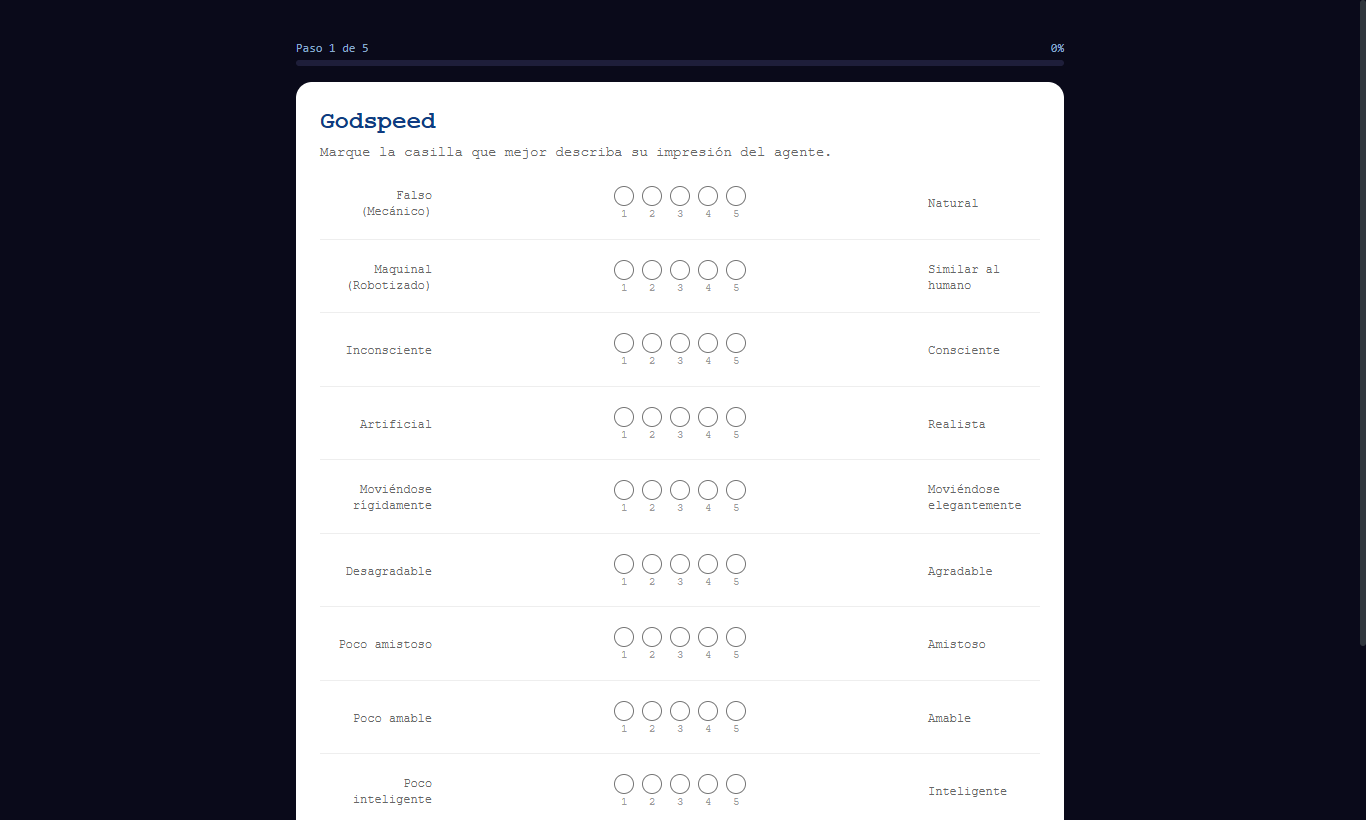
\includegraphics[width=\columnwidth]{figures/questionnaire.png}
  \caption{Ejemplo de instrumento (Godspeed) administrado en la aplicaci\'on al final de la
  interacci\'on, con barra de progreso del conjunto de cuestionarios.}
  \label{fig:quest}
\end{figure}

\paragraph{Verificaci\'on de la manipulaci\'on}
La condici\'on se aplica en el servidor y determina de forma determinista la interfaz: la
Condici\'on~A habilita el avatar Kaplay, la voz Piper/STT y la gamificaci\'on por anillos, mientras
que la Condici\'on~B las elimina por completo; el \emph{texto} del tutor es id\'entico en ambas.
As\'i, cualquier diferencia observada es atribuible al \emph{embodiment} y no al contenido del
tutor.

\begin{table}[t]
  \caption{Conjunto de instrumentos. En el piloto entre-sujetos se aplica una
  sola vez al final; en el dise\~no \emph{crossover} refinado, los instrumentos
  espec\'ificos de condici\'on (Godspeed, apoyo pedag\'ogico, SUS, NASA-TLX,
  PANAS-SF) se aplican una vez por bloque y los dem\'as una sola vez.}
  \label{tab:instruments}
  \centering
  \footnotesize
  \begin{tabular}{@{}lll@{}}
    \toprule
    \textbf{Instrumento} & \textbf{Constructo} & \textbf{RQ} \\
    \midrule
    Demogr\'aficos & Perfil de la muestra & --- \\
    Godspeed~\cite{bartneck2009godspeed} & Antropomorfismo, agrado & RQ1 \\
    Apoyo pedag\'ogico (5 \'items)~\cite{essel2024aimediated} & Apoyo socr\'atico percibido & RQ1 \\
    SUS~\cite{brooke1996sus} & Usabilidad & RQ1 \\
    NASA-TLX~\cite{hart1988nasatlx} & Carga cognitiva (RTLX) & RQ3 \\
    PANAS-SF~\cite{thompson2007ipanas} & Afecto post-sesi\'on & RQ3 \\
    Preguntas abiertas & Apreciaci\'on cualitativa & --- \\
    Telemetr\'ia autom\'atica & Eficacia, latencia & RQ2, RQ4 \\
    \bottomrule
  \end{tabular}
\end{table}

\subsection{Protocolo de interacci\'on}
Protocolo ejecutado en el piloto (entre-sujetos): (1) el participante pulsa \emph{PRESS START} y el
servidor asigna condici\'on e identificador an\'onimo; (2) resuelve la Tarea~1 (m\'ax.\ 10~min)
interactuando por texto (ambas condiciones) o voz (Condici\'on~A); (3) mini-juego de transici\'on;
(4) resuelve la Tarea~2 (m\'ax.\ 10~min); (5) completa los cuestionarios finales. El tutor aplica
andamiaje de tres niveles y env\'ia mensajes proactivos tras 60~s de inactividad, sin entregar
c\'odigo. En el protocolo \emph{crossover} refinado, este ciclo de dos tareas se repite en la
condici\'on opuesta (con las variantes de tarea) y el conjunto de cuestionarios espec\'ifico de la
condici\'on se
responde al final de cada bloque.

\subsection{Recolecci\'on de datos}
El flujo de recolecci\'on (Fig.~\ref{fig:flow}) es totalmente automatizado: desde la asignaci\'on
en el servidor hasta la persistencia y exportaci\'on, sin intervenci\'on manual que introduzca
errores de transcripci\'on. Cada sesi\'on se guarda en una base de datos SQLite local bajo un
identificador an\'onimo (\texttt{P-001}, \dots), sin nombre ni correo. El sistema exporta un CSV con
una fila por participante (ver el diccionario de datos del repositorio), un JSON de fidelidad
completa y las transcripciones de conversaci\'on en JSONL para la codificaci\'on cualitativa.

\begin{figure}[t]
  \centering
  \footnotesize
  \begin{tikzpicture}[
    node distance=2.4mm and 4mm,
    step/.style={draw, rounded corners=2pt, fill=blue!7, align=center, font=\scriptsize,
                 inner sep=3pt, text width=15mm, minimum height=8mm},
    store/.style={draw, fill=green!10, align=center, font=\scriptsize, inner sep=3pt,
                  text width=15mm, minimum height=8mm},
    >={Stealth[length=1.6mm]}]
    \node[step] (assign) {Asignaci\'on (servidor)};
    \node[step, right=of assign] (inter) {Interacci\'on tutor + tareas};
    \node[step, right=of inter] (quest) {Cuestionarios};
    \node[store, right=of quest] (db) {SQLite \texttt{sonic.db}};
    \node[step, below=6mm of db] (panel) {Panel del facilitador};
    \node[store, left=of panel] (export) {Export CSV / JSON / JSONL};
    \node[step, left=of export] (analysis) {An\'alisis (\emph{script})};
    \draw[->] (assign) -- (inter);
    \draw[->] (inter) -- (quest);
    \draw[->] (quest) -- (db);
    \draw[->] (db) -- (panel);
    \draw[->] (db) -- (export);
    \draw[->] (export) -- (analysis);
    \draw[->] (db.north) to[out=110,in=70] node[above,font=\scriptsize] {telemetr\'ia continua} (inter.north);
  \end{tikzpicture}
  \caption{Flujo de recolecci\'on y an\'alisis de datos, de extremo a extremo.}
  \label{fig:flow}
\end{figure}

El an\'alisis descriptivo por condici\'on est\'a disponible en vivo en el \textbf{panel del
facilitador} (Fig.~\ref{fig:admin}), que muestra el balance A/B, gr\'aficos comparativos y la tabla
de estad\'isticas; el an\'alisis inferencial (Mann--Whitney $U$, $\delta$ de Cliff, $d$ de Cohen) se
ejecuta sobre el CSV con el \emph{script} incluido en el repositorio.

\begin{figure}[t]
  \centering
  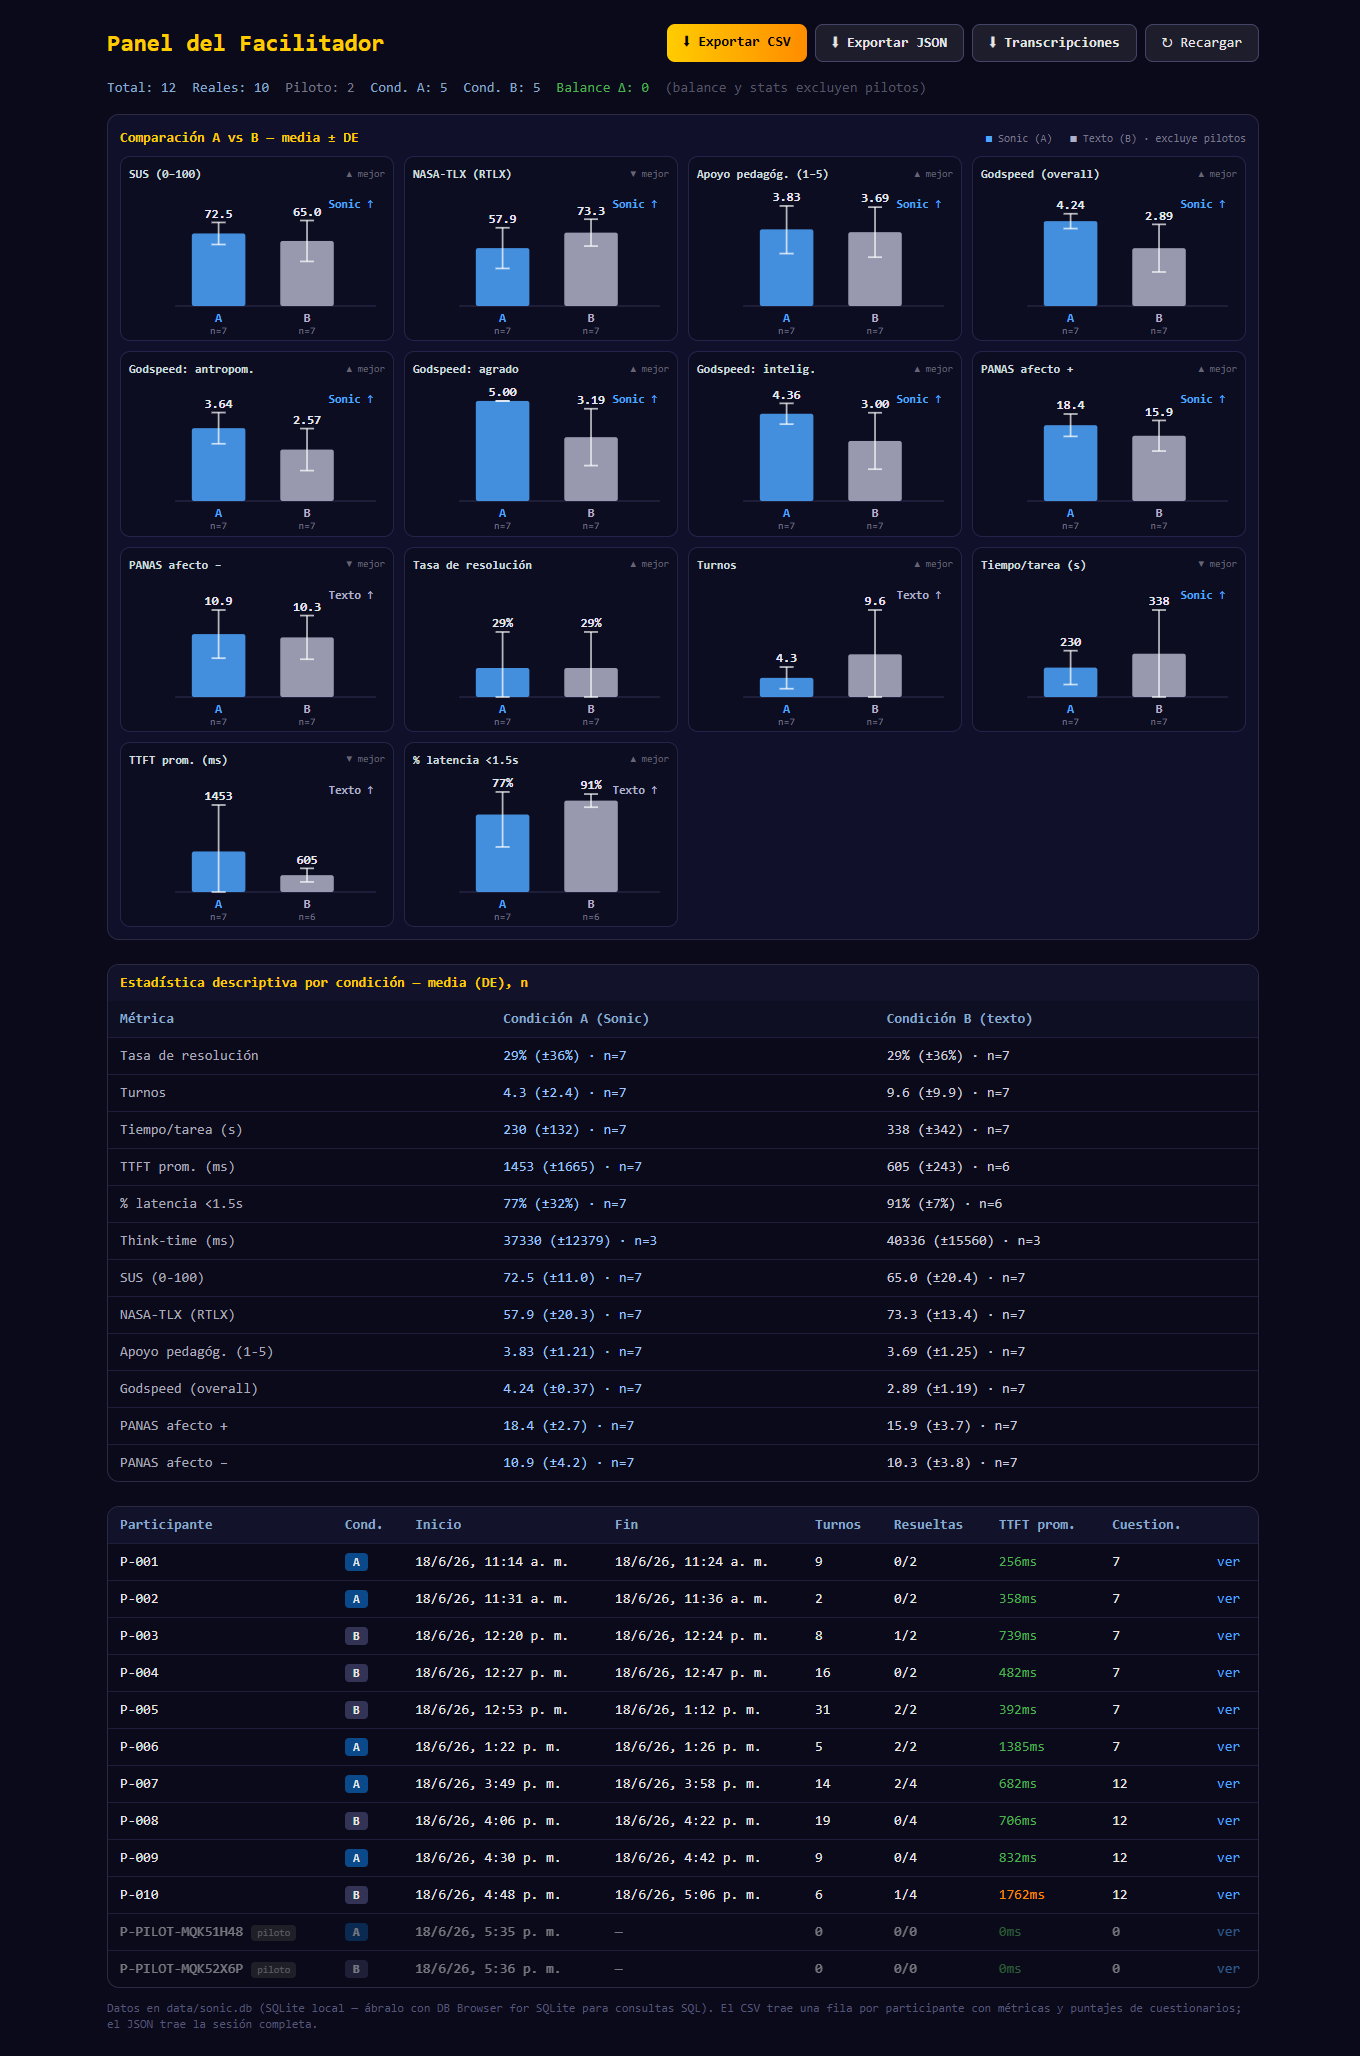
\includegraphics[width=\columnwidth]{figures/admin.png}
  \caption{Panel del facilitador (programa real): balance por condici\'on, gr\'aficos comparativos
  A vs.\ B, estad\'istica descriptiva y listado de participantes; los pilotos se excluyen de los
  estad\'isticos.}
  \label{fig:admin}
\end{figure}

%--------------------------------------------------------------
\section{Resultados}
\label{sec:results}
Se reportan estad\'isticas descriptivas por condici\'on (media, DE) y, dado el tama\~no muestral
reducido (7 observaciones por condici\'on), se prioriza el \textbf{tama\~no de efecto} ($d$ de
Cohen; $A-B$) sobre la significancia inferencial. La Tabla~\ref{tab:results} resume las m\'etricas
principales. La unidad del contraste es la \emph{observaci\'on por condici\'on}: cada participante
\emph{crossover} aporta una observaci\'on a cada condici\'on y cada participante entre-sujetos una a
su condici\'on, totalizando 7 en A y 7 en B. La Figura~\ref{fig:results} ilustra la pantalla de
resultados que cierra cada sesi\'on, con las cuatro corridas etiquetadas por condici\'on en el
dise\~no \emph{crossover}.

\begin{figure}[t]
  \centering
  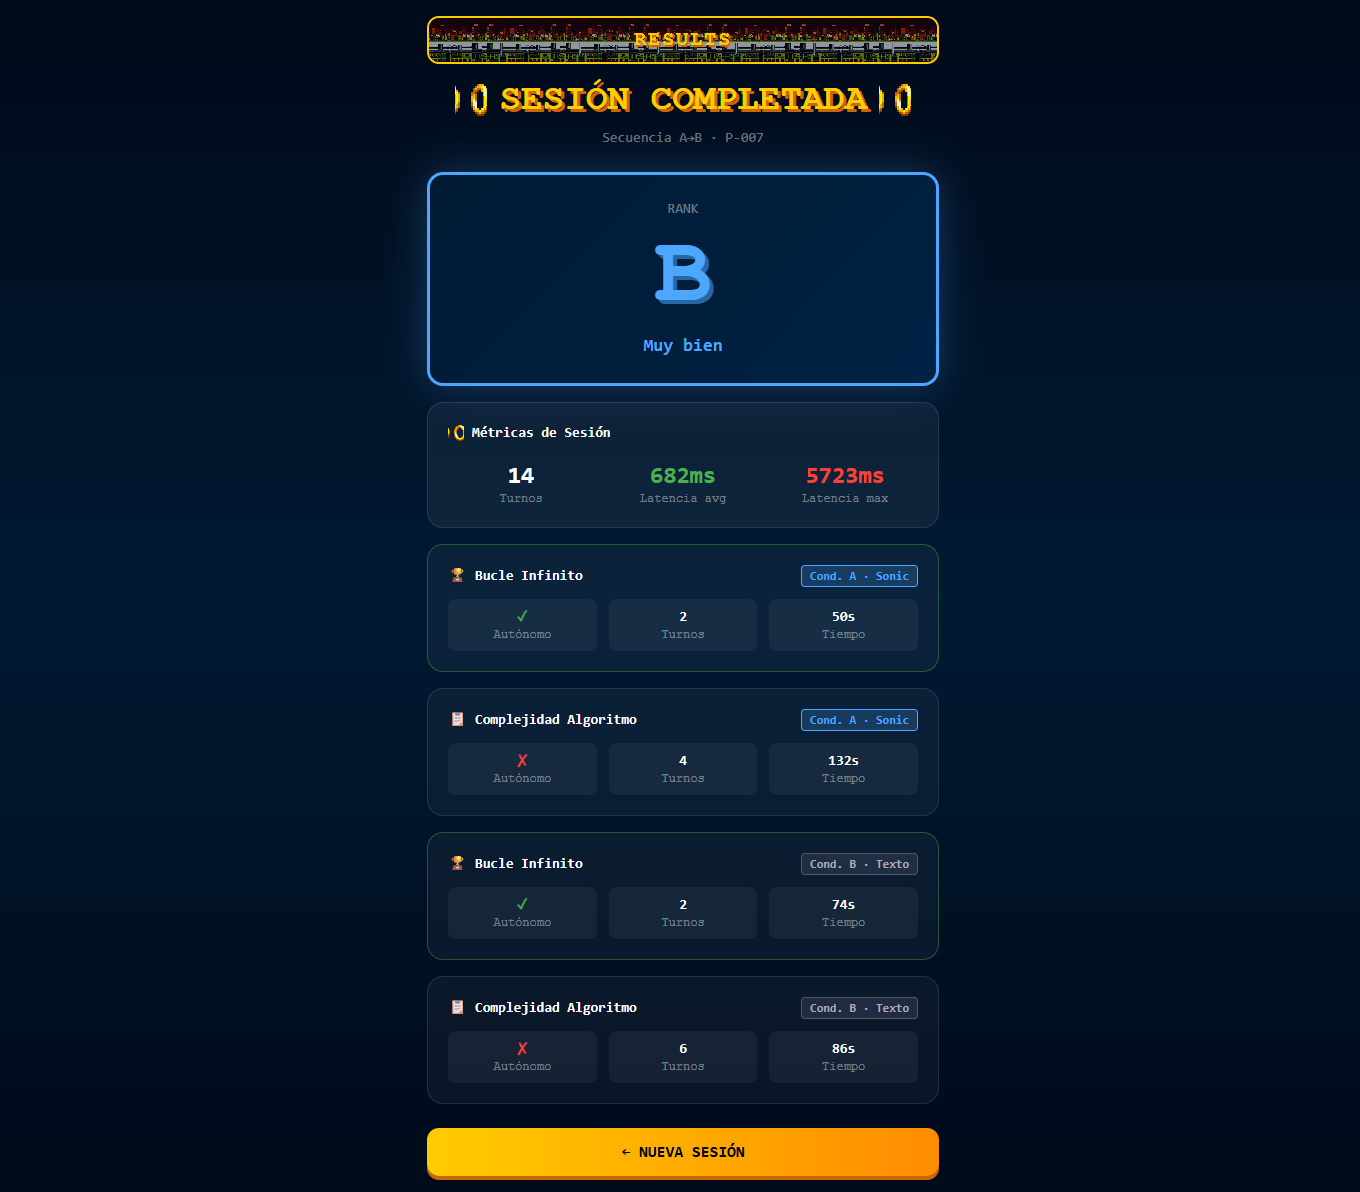
\includegraphics[width=0.82\columnwidth]{figures/results.png}
  \caption{Pantalla de resultados de una sesi\'on \emph{crossover} (P-007, secuencia A$\to$B): rango
  resumen, m\'etricas de sesi\'on y las cuatro corridas (ambas tareas en cada condici\'on) con su
  etiqueta de condici\'on.}
  \label{fig:results}
\end{figure}

\begin{table}[t]
  \caption{Resultados descriptivos por condici\'on, media (DE), 7 observaciones cada una.
  $d$: tama\~no de efecto de Cohen ($A-B$); ${}^{*}p<0{,}05$ (Mann--Whitney). En \emph{Turnos},
  \emph{Tiempo} y \emph{NASA-TLX} un valor menor es mejor.}
  \label{tab:results}
  \centering
  \footnotesize
  \begin{tabular}{@{}lccc@{}}
    \toprule
    \textbf{M\'etrica} & \textbf{Cond.\ A} & \textbf{Cond.\ B} & \textbf{$d$} \\
    \midrule
    Resoluci\'on aut\'onoma (0--1) & 0{,}29 (0{,}39) & 0{,}29 (0{,}39) & $0{,}00$ \\
    Turnos por tarea & 3{,}4 (1{,}6) & 5{,}7 (5{,}1) & $-0{,}60$ \\
    Tiempo por tarea (s) & 230 (143) & 338 (369) & $-0{,}39$ \\
    TTFT mediano (ms) & 218 & 244 & --- \\
    \% latencia $<1.5$\,s & 88 & 94 & --- \\
    SUS (0--100) & 72{,}5 (11{,}9) & 65{,}0 (22{,}1) & $0{,}42$ \\
    Apoyo pedag\'ogico (1--5) & 3{,}83 (1{,}30) & 3{,}69 (1{,}35) & $0{,}11$ \\
    NASA-TLX (RTLX) & 57{,}9 (22{,}0) & 73{,}3 (14{,}5) & $-0{,}83$ \\
    Godspeed global (1--5) & 4{,}24 (0{,}40) & 2{,}89 (1{,}29) & $1{,}42$ \\
    \quad\emph{antropomorfismo} & 3{,}64 (0{,}84) & 2{,}57 (1{,}13) & $1{,}07$ \\
    \quad\emph{agrado}${}^{*}$ & 5{,}00 (0{,}00) & 3{,}19 (1{,}54) & $1{,}66$ \\
    \quad\emph{inteligencia} & 4{,}36 (0{,}56) & 3{,}00 (1{,}53) & $1{,}18$ \\
    PANAS afecto $+$ & 18{,}4 (2{,}9) & 15{,}9 (4{,}0) & $0{,}73$ \\
    PANAS afecto $-$ & 10{,}9 (4{,}5) & 10{,}3 (4{,}1) & $0{,}13$ \\
    \bottomrule
  \end{tabular}
\end{table}

\paragraph{Percepci\'on del agente (RQ1)} La corporizaci\'on produjo el efecto m\'as grande y
consistente: Godspeed global fue muy superior en A (4{,}24 vs.\ 2{,}89; $d=1{,}42$; $p=0{,}055$),
y la subescala de \emph{agrado} alcanz\'o significancia pese al tama\~no muestral (5{,}00 vs.\
3{,}19; $d=1{,}66$; $\delta$ de Cliff${}=0{,}71$; $p=0{,}011$), con antropomorfismo e inteligencia
tambi\'en favorables a A ($d=1{,}07$ y $1{,}18$). La usabilidad (SUS) fue solo ligeramente mayor en
A ($d=0{,}42$) y el apoyo pedag\'ogico percibido fue equivalente ($d=0{,}11$), lo que sugiere que el
efecto se concentra en la \emph{presencia social} del avatar y no en una interfaz m\'as usable ni en
una percepci\'on distinta del andamiaje.

\paragraph{Eficacia aut\'onoma (RQ2)} La tasa de resoluci\'on aut\'onoma fue id\'entica entre
condiciones (0{,}29 en ambas; $d=0$). La Condici\'on~A requiri\'o algo menos de turnos por tarea
(3{,}4 vs.\ 5{,}7; $d=-0{,}60$) y de tiempo ($d=-0{,}39$), pero con esta muestra y la heterogeneidad
de experiencia previa no puede atribuirse causalidad al \emph{embodiment}.

\paragraph{Carga cognitiva y afecto (RQ3)} La carga autopercibida (NASA-TLX) fue \emph{menor} en A
(57{,}9 vs.\ 73{,}3; $d=-0{,}83$) y el afecto positivo (PANAS) mayor ($d=0{,}73$), sin diferencia
relevante en afecto negativo. Es decir, en este piloto la corporizaci\'on no aument\'o la carga
---el riesgo advertido por~\cite{li2025cognitiveload}--- sino que acompa\~n\'o a una experiencia
percibida como m\'as ligera y positiva.

\paragraph{Latencia (RQ4)} Sobre 119 respuestas del tutor, el \emph{time-to-first-token} se mantuvo
bajo 1.5~s en el 92\,\% de los casos (mediana 234~ms). El cumplimiento fue algo menor en la
Condici\'on~A (88\,\% vs.\ 94\,\%), atribuible a respuestas ocasionalmente m\'as lentas en las
sesiones con voz y avatar y en las realizadas de forma remota; aun as\'i, la mediana de A (218~ms)
fue equivalente, confirmando la viabilidad del objetivo de latencia con inferencia local.

\subsection{Hallazgos cualitativos}
El an\'alisis tem\'atico de las respuestas abiertas (codificadas seg\'un el esquema del
repositorio) revel\'o patrones coherentes con los cuantitativos:
\begin{itemize}
  \item \textbf{Preferencia por la corporizaci\'on, incluso intra-sujeto.} El testimonio m\'as
        fuerte proviene de participantes \emph{crossover} que vivieron ambas condiciones:
        \emph{``El chat de texto fue molesto y poco pr\'actico\ldots no veo que el sistema est\'e
        interactuando conmigo''} y \emph{``Prefiero 100\,\% el usar la opci\'on del avatar de Sonic
        mientras aprendo algo tan dif\'icil como\ldots\ programar''} (P-007). En la fase
        entre-sujetos, quienes solo tuvieron texto tambi\'en pidieron el avatar:
        \emph{``No me gust\'o no ver a Sonic''} (P-005); \emph{``Prefiero el aprender junto con un
        agente virtual como Sonic''} (P-003). Ning\'un participante expres\'o la preferencia
        inversa.
  \item \textbf{Presencia social y gu\'ia percibida.} Se valor\'o la reactividad del avatar:
        \emph{``poder charlar con Sonic y ver c\'omo este reaccionaba ante mis comentarios. Fue una
        gu\'ia para m\'i''} (P-006); \emph{``es Sonic\ldots lo que lo hace m\'as interactivo''}
        (P-008); \emph{``es amable, amigable y divertido''} (P-002).
  \item \textbf{El andamiaje socr\'atico se percibi\'o.} Un participante de texto destac\'o
        \emph{``que de verdad me fuera ayudando\ldots sin darme la respuesta''} (P-005),
        evidenciando que la restricci\'on de no entregar c\'odigo fue percibida como apoyo y no
        como carencia.
  \item \textbf{Presi\'on de la gamificaci\'on.} Un participante report\'o
        \emph{``un poco de presi\'on para contestar r\'apido, porque sent\'ia que pod\'ia perder el
        nivel''} (P-009), se\~nal de que el sistema de anillos puede a\~nadir demanda temporal ---un
        matiz relevante para la carga cognitiva (RQ3).
  \item \textbf{Fricciones de usabilidad y prerrequisitos.} Se mencionaron el tiempo de respuesta y
        la falta de explicaci\'on inicial de los controles (P-002), y la barrera de conocimiento
        previo en participantes sin experiencia (\emph{``como no s\'e nada sobre programaci\'on me
        tom\'o m\'as tiempo entender el c\'odigo''}, P-009; similar en P-001).
  \item \textbf{Efecto de repetici\'on.} Un participante de la Fase~1 se\~nal\'o que repetir el
        mismo ejercicio no aportaba (\emph{``no me gust\'o volver a hacer las mismas preguntas''},
        P-006), hallazgo que motiv\'o directamente las variantes de tarea introducidas en la
        Fase~2.
\end{itemize}

%--------------------------------------------------------------
\section{An\'alisis y Discusi\'on}
\label{sec:discussion}
Los resultados del piloto, aunque preliminares, dibujan un patr\'on coherente entre las medidas
cuantitativas y cualitativas. Respecto a \textbf{RQ1}, la corporizaci\'on elev\'o de forma
sustancial la percepci\'on del agente (Godspeed global $d=1{,}42$; agrado $d=1{,}66$ con
$p=0{,}011$) con solo una mejora menor de usabilidad ($d=0{,}42$) y sin diferencia en el apoyo
pedag\'ogico percibido ($d=0{,}11$): el efecto se concentra en la \emph{presencia social} del
avatar y la voz, no en una interfaz m\'as f\'acil ni en una percepci\'on distinta del andamiaje.
Esto concuerda con los efectos de presencia social reportados en agentes
corporizados~\cite{elhajji2025architecture,sonlu2024scoping} y se ve reforzado por el dato
cualitativo m\'as fuerte: participantes que experimentaron \emph{ambas} condiciones prefirieron sin
ambig\"uedad el avatar sobre el texto.

En cuanto a \textbf{RQ3}, la condici\'on corporizada se asoci\'o a una carga cognitiva
autopercibida \emph{menor} (NASA-TLX, $d=-0{,}83$) y a un afecto positivo mayor ($d=0{,}73$). Es
decir, en este contexto no se materializ\'o el riesgo de que el agente \emph{aumente} la carga en
tareas densas advertido por~\cite{li2025cognitiveload}; una interpretaci\'on plausible es que la
voz y el andamiaje visual redujeron la carga \emph{extr\'inseca} de la interacci\'on. No obstante,
un participante report\'o sentir presi\'on temporal por el sistema de anillos, lo que sugiere que la
gamificaci\'on puede introducir demanda adicional y debe calibrarse. Para \textbf{RQ2}, la eficacia
de resoluci\'on fue \emph{id\'entica} entre condiciones ($d=0$): la corporizaci\'on mejor\'o la
experiencia sin penalizar (ni, en este piloto, potenciar) el desempe\~no objetivo. Finalmente,
\textbf{RQ4} se cumpli\'o: 92\,\% de las respuestas bajo 1.5~s con inferencia totalmente local
(mediana 234~ms), con un cumplimiento algo menor en la Condici\'on~A por respuestas puntuales m\'as
lentas en sesiones con voz y remotas.

Coherente con la d\'ebil correlaci\'on entre auto-reporte y conducta~\cite{dang2020selfreport} y
con la recomendaci\'on de no depender de los cuestionarios ante $N$ peque\~no, la evidencia m\'as
robusta de este piloto proviene de la \emph{convergencia} entre el efecto de percepci\'on
(Godspeed, con agrado significativo), la se\~nal conductual (menos turnos) y la preferencia
expl\'icita ---incluso intra-sujeto--- por la corporizaci\'on en las respuestas abiertas.

\paragraph{Limitaciones}
Las conclusiones son preliminares y deben leerse con cautela. (i)~\emph{Tama\~no muestral}: con 7
observaciones por condici\'on los intervalos de confianza son amplios; aunque la subescala de
agrado alcanz\'o significancia, la mayor\'ia de los efectos no, y sus magnitudes pueden variar con
m\'as datos. (ii)~\emph{Dise\~no mixto y confusi\'on}: parte de la evidencia proviene de
comparaciones entre-sujetos donde la experiencia previa no qued\'o balanceada, por lo que las
diferencias de eficacia (RQ2) no son atribuibles limpiamente al \emph{embodiment}; el dise\~no
\emph{crossover} (Fase~2) mitiga esto y se propone como dise\~no principal a escala.
(iii)~\emph{Homogeneidad de la muestra}: predominio de hombres j\'ovenes (9 de 10), lo que limita la
generalizaci\'on. (iv)~\emph{Efecto de novedad}: la valoraci\'on de la Condici\'on~A pudo inflarse
por la familiaridad y el atractivo del personaje Sonic, un efecto que suele atenuarse con el uso
repetido. (v)~\emph{Medici\'on \emph{post-only}} del afecto (sin l\'inea base) y \emph{dependencia
del hardware} y la red para la latencia.

%--------------------------------------------------------------
\section{Conclusiones y Trabajo Futuro}
\label{sec:conclusion}
Se present\'o \emph{Sonic}, un tutor socr\'atico multimodal corporizado, completamente local y
reproducible, junto con un dise\~no que a\'isla el \emph{embodiment} (texto de tutor id\'entico) y
verifica la autonom\'ia con pruebas ocultas en lugar de auto-reporte. La evidencia del estudio
piloto ($N=10$), aunque preliminar, es internamente coherente: la corporizaci\'on se asoci\'o a una
percepci\'on del agente notablemente mejor (Godspeed global $d=1{,}42$; agrado $d=1{,}66$,
$p=0{,}011$) y a una carga cognitiva autopercibida menor (NASA-TLX, $d=-0{,}83$), con eficacia de
resoluci\'on equivalente, mientras la latencia local cumpli\'o el objetivo ($<1.5$~s en el 92\,\%
de las respuestas). El dato cualitativo m\'as claro ---que los participantes, incluidos quienes
vivieron ambas condiciones, prefirieran el avatar--- converge con la se\~nal cuantitativa de
presencia social. La principal conclusi\'on, por tanto, es que el \emph{embodiment} parece operar
sobre la dimensi\'on socio-afectiva y de carga percibida sin penalizar la eficacia, lo que
justifica un estudio confirmatorio con mayor poder. El trabajo
futuro incluye la ejecuci\'on del dise\~no \emph{crossover} con variantes de tarea aqu\'i descrito,
planificaci\'on adaptativa del di\'alogo~\cite{dong2026learning}, m\'as tareas y dominios, y una
muestra mayor y m\'as diversa.

\paragraph{Proyecci\'on de publicaci\'on}
S\'i se proyecta dar continuidad a este trabajo. Se planea ejecutar el estudio completo con el
dise\~no intra-sujeto (\emph{crossover}) y las variantes de tarea ya implementadas en el sistema,
ampliando la muestra y su diversidad, previo sometimiento y aprobaci\'on del Comit\'e \'Etico
Cient\'ifico (CEC) de la Universidad de Costa Rica, con miras a una eventual publicaci\'on
acad\'emica. La presente entrega constituye el piloto de viabilidad que fundamenta dicha
proyecci\'on.

%--------------------------------------------------------------
\section*{Disponibilidad}
El c\'odigo fuente, las instrucciones de reproducci\'on y el video de demostraci\'on est\'an
disponibles en el repositorio del proyecto.

\bibliographystyle{IEEEtran}
\bibliography{references}

\end{document}
